\documentclass{article}
\usepackage{amssymb}
\usepackage{geometry}
\geometry{margin=1.5in}
\usepackage{graphicx}
\graphicspath{{img/}}
\begin{document}

We want to find function $f$ from class $\mathcal{F}$, which we call the
\textbf{hypothesis class}.

\smallskip

We choose a \textbf{loss function} to measure how well $f$ does at the learning
problem.

\smallskip

\textbf{Risk} or \textbf{expected loss} is:

$$
R(f) = E(X,Y) \sim_P[L(Y, f(x))]
$$
or
$$
R(f) = E(X) \sim_P[L(X, f(x))]
$$

\smallskip

We denote the optimal risk as $r^*$ and the optimal function as $f^*$

\smallskip

The Bayes classifier, $f^*(x) = argmax_y P(Y=y|X=x)$, is the theoretical optimum
(at least for 0-1 loss). But, it isn't a practical scheme because we don't
actually know the conditional distribution. Rather, we use it as a benchmark.

\smallskip

We have a host of \textbf{margin-based} loss functions (margin is
$yf(\mathbf{X})$ for $\mathbf{X} \in \mathbb{R}, y \in {-1,1}$). The margin only
takes positive values when the classification is correct. A margin-based
loss function is: $L(y, f(x)) = L(yf(x))$. The simple 0-1 loss function can be
written as $I(yf(x) < 0$ (we want to minimize this). We are interested in
alternate loss functions that have two key properties:
\begin{itemize}
	\item $L$ is a convex function of the margin
	\item $L$ upper bounds $L_{0-1}$ (our above simple 0-1 loss function)
\end{itemize}

\smallskip

Some candidate functions (for classification) are below. All of them have the
same sign as Bayes loss and so are called \textbf{classification-calibrated} or
\textbf{surrogate} loss functions, in that minimizing them is equivalent to
minimizing Bayesian loss.

\begin{table}[h]
	\centering
	\begin{tabular}{|c | c | c|}
		\hline
		\textbf{Loss function} & \textbf{Form} & \textbf{Notes}\\
		Hinge & $\mathrm{max}\{0, 1-yf(x)\}$ & Tightest convex upper bound to 0-1; non-smooth\\
		Exponential &  $ \mathrm{exp}(-yf(x))$ & 1-Lipschitz (robust)\\
		Logistic & $ \mathrm{log}_2(1+\exp(-yf(x)))$ & 1-Lipschitz (robust)\\
		Squared & $(1-yf(x))^2$ & Not recommended for class. (weird errors)\\
		Squared hinge &  $\mathrm{max}\{0, 1-yf(x)\}^2$ & Only 1x differentiable
		at 1\\
		\hline
	\end{tabular}
\end{table}
\begin{centering}
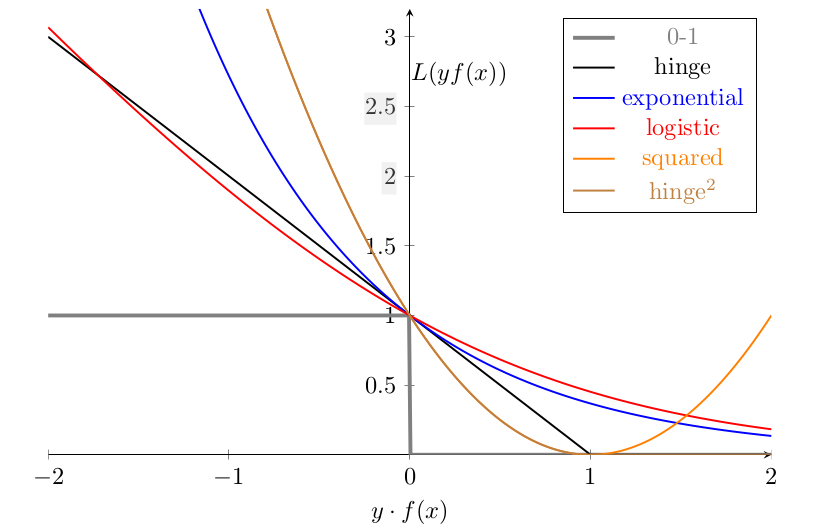
\includegraphics[scale=0.35]{graph}
\end{centering}

Now, let's switch from classification to regression. Some potential loss
functions are:

\begin{table}[h]
	\centering
	\begin{tabular}{|c | c |}
		\hline
		\textbf{Loss function} & \textbf{Form} \\
		Squared & $(y-f(x))^2$  \\
		Absolute & $L_1(y, f(x)) = |y-f(x)|$\\
		$\epsilon$-insensitive & $|y-f(x)|I(|y-f(x)|\geq \epsilon)$ \\
		Huber & loooong \\
		\hline
	\end{tabular}
\end{table}

\begin{centering}
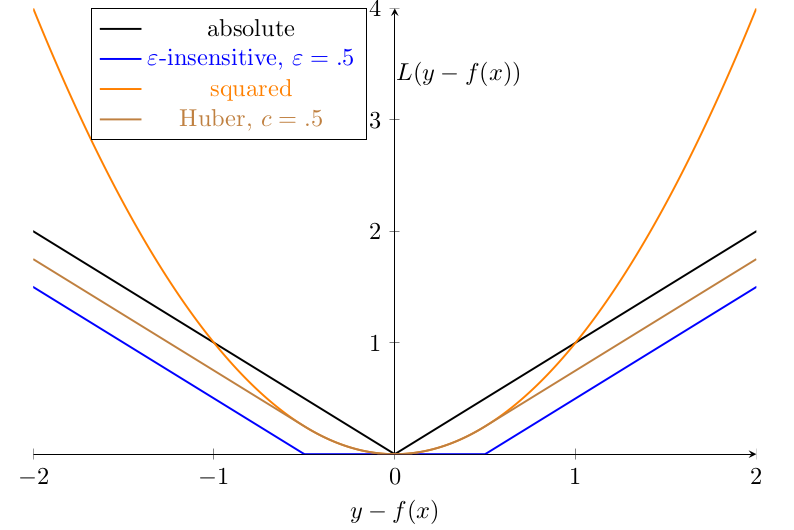
\includegraphics[scale=0.35]{graph2}
\end{centering}

We want minimize risk (expected loss) ($E_{(X,Y)\sim_P[L(Y, f(X))]}$) over all
possible $f$. But that's ambitious, so lets replace $R$ by its empirical
counterpart:

$$
R_{\mathrm{emp}} (f) = \frac{1}{n} \sum_{i=1}{n} L(Y_i, f(X_i))
$$

By LLN, we know that for any \textbf{fixed} f, $R_{\mathrm{emp}}(f) \to R(f)$ as
$n \to \infty$, but we can't be assured that we have infinite $n$, nor is $f$
fixed (we are considering lots of $f$), so this is a weak guarantee. Let $\mathcal{F}$ be the hypothesis class the minimum is taken over:

$$
\mathrm{min}_{f \in \mathcal{F}} R_{\mathrm{emp}}(f)
$$

Denote empirical risk minimizer as $\hat{f}$. Denote minimizer of risk over the
class $\mathcal{F}$ as $\bar{f}$. The difference between the minimum risk $\bar{R}$ over $\mathcal{F}$ and the
minimum risk $R^*$ is called \textbf{excess risk}. Reminder: $R(f^*)$ is
theoretical optimum. Theorem:
$$R(\hat{f}) \leq R(\bar{f}) + 2 \mathrm{sup}_{f \in
\mathcal{F}}|R_\mathrm{emp}(f)-R(f)|$$
$$= R(f^*) + \epsilon(\bar{f}) + 2 \mathrm{sup}_{f \in
\mathcal{F}}|R_\mathrm{emp}(f)-R(f)|$$
$$
= \mathrm{intrinsic error} + \mathrm{approximation error} + \mathrm{estimation
error}
$$

The latter two are bias and variance by another name. They are antagonists:
decreasing one means increasing another. 

\smallskip

You can fit any series of datapoints with interpolating polynomial of degree
$n-1$. You are guaranteed to minimize empirical risk, but it will generalize
poorly to new data. Or, you can have some really general method, but it will
have high empirical risk.

\smallskip

A good way to find the optimal balance is \textbf{regularization}, covered next
class.

\end{document}
